\label{ch:conclusiones}

%Algo de texto...

\section{Comparación de Resultados}\label{sec:comparativa}

En este apartado se lleva a cabo la comparación de resultados entre los
obtenidos en las simulaciones CFD y los experimentales. Como ya se ha
descrito, las limitaciones geométricas y de los aparatos de medida
condicionarán los ensayos para el uso de los diafragmas de diámetros
{[}13-14-15,5-16{]}mm. Es decir, por una parte el medidor de presión
estática está limitado a 100Pa y el diámetro interior de la tubería que
hace de chimenea es de 19,6mm.

Por lo tanto, los valores
obtenidos que se tendrán en cuenta para validar las simulaciones
realizadas por ordenador con el canal 3-D del laboratorio, se recopilan en la \autoref{tab:cfd} para las simulaciones y en la \autoref{tab:exp} los del ensayo.

\begin{table}
\centering
\caption{Resultados para la simulación de lo 4 últimos casos}
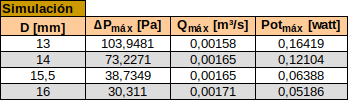
\includegraphics[width=0.55\linewidth]{TabCFD.png}
\label{tab:cfd}
\end{table}

\begin{table}
\centering
\caption{Resultados hallados de la experimentación en el
canal del laboratorio}
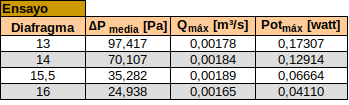
\includegraphics[width=0.55\linewidth]{TabEXP.png}
\label{tab:exp}
\end{table}

A partir de esto, se puede calcular el porcentaje de error para comparar
cómo de exactos son los valores de las simulaciones por ordenador
respecto del valor real medido experimentalmente, \autoref{tab:porcentajeError}

\begin{table}
\centering
\caption{Porcentajes de error entre el ensayo y las simulaciones}
\label{tab:porcentajeError}
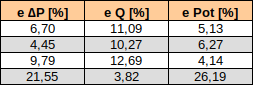
\includegraphics[width=0.4\linewidth]{porcentajeError.png}
\end{table}

A continuación, se analizan los resultados para cada una de las
variables:

\begin{figure}
\centering
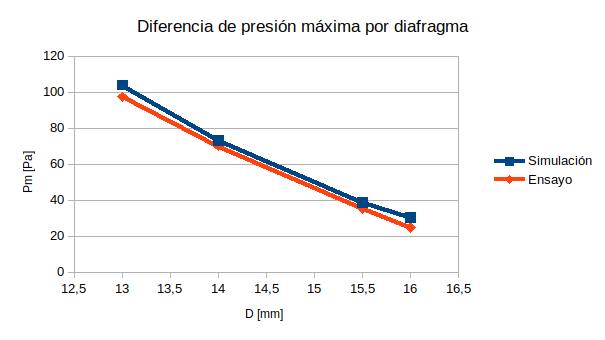
\includegraphics[width=0.7\linewidth]{PDiaf.png}
\caption[Presión máxima aguas arriba del diafragma]{Representación de la máxima presión hallada aguas arriba del diafragma}
\label{fig:PDiaf}
\end{figure}

\begin{figure}
  \centering
  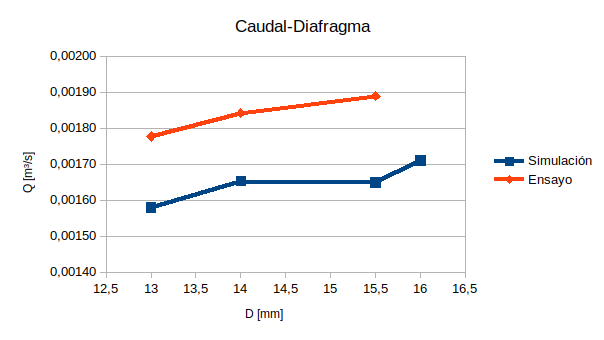
\includegraphics[width=0.7\linewidth]{QDiaf.png}
  \caption[Gráfica comparación de caudal máximo]{Gráfico del caudal máximo para cada diafragma}
  \label{fig:QDiaf}
  \end{figure}

\begin{itemize}
\item
  \textbf{Altura del agua dentro de la cámara:}

  El resultado obtenido de la altura del agua dentro de la cámara para
  cada caso, se extrae de la tabla, ya que este valor permanece
  prácticamente constante independientemente del diafragma que se
  utilice.

  Por un lado, para todas las simulaciones, el máximo valor alcanzado es
  de \(0,24m\), a este valor se le resta \(0,075m\), valor
  correspondiente a la distancia desde el origen de coordenadas hasta el
  fondo del canal, quedando en una altura máxima de \(0,165m\).
  Encambio, para las pruebas ensayadas se tiene una mayor incertidumbre
  en la exactitud de la medición, tomando como valor medio el rango de
  \((0,155-0,165)m\).

  Con estos valores, se concluye que los resultados obtenidos por ambas
  vías, prácticamente resultan iguales.
\item
  \textbf{Diferencia de presiones máximas a la salida de la chimenea:}

  Por un lado, se comparan los máximos alcanzados por cada diafragma,
  comprobando que los valores hallados permanecen bastante parejos, ver la gráfica \autoref{fig:PDiaf}.

  Por otro lado, en la gráfica \autoref{fig:potTCanal3D} del apartado \ref{sec:canal3d}, además de representar los
  resultados del ensayo para cada diafragma, se añade la curva de las
  simulaciones correspondiente a ese mismo rango. Como se puede
  apreciar, los resultados son bastante satisfactorios, coincidiendo en
  gran medida, salvo para el caso del diafragma de \(16mm\).

  En este último caso, se supera el 20\% del error en la medida. Esto
  puede ser porque, al ser el diámetro interior de la chimenea de
  \(19,6mm\), el aire apenas se ve comprimido cuando el agua entra a la
  cámara. Dando lugar a una presión de flujo menos apreciable aún, en el
  caso de la experimentación.

  Asimismo, en la subapartado \ref{header-n277}, donde se describían las placas de orificio, se
  define el rango límite que la normativa establece para la relación de
  diámetros de \(\beta\), del cual, este diafragma, queda fuera. Es
  probable que para evitar errores en las mediciones, se prevenga
   dicho límite.
\item
  \textbf{Caudal a través del diafragma:}

  Estos resultados, representados en la gráfica \autoref{fig:QDiaf}, son los que más difieren entre sí, aun así la escala
  es muy pequeña y el error que se da es de alrededor del 10\%, esto
  puede deberse a que en el ensayo no fue posible garantizar un volumen
  de agua exacto para todas las pruebas.
\item
  \textbf{Potencia en función del diafragma:}

  Como para los valores anteriores, como puede verse en la gráfica \autoref{fig:PotDiaf}, estos también se asemejan entre sí
  en gran medida.
\end{itemize}

\begin{figure}
\centering
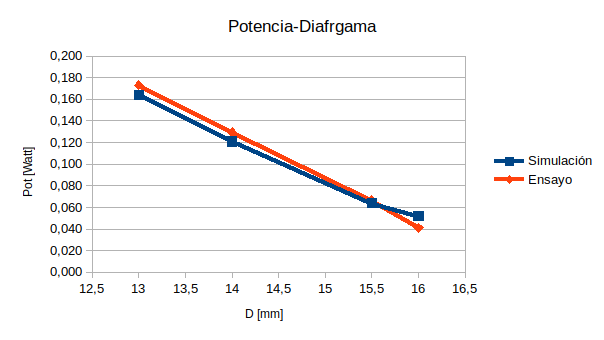
\includegraphics[width=0.7\linewidth]{PotDiaf.png}
\caption{Potencia máxima para cada diagrama}
\label{fig:PotDiaf}
\end{figure}

\section{Conclusión final}\label{sec:conclusion}

Teniendo en cuenta los propósito establecidos al comienzo de este
proyecto, las fases abordadas y los resultados obtenidos se concluye con
lo siguiente:

\begin{enumerate}
\def\labelenumi{\arabic{enumi}.}
\item
  Con este estudio se valida la representación del principio de
  funcionamiento del prototipo OWC computacional y experimentalmente.
\item
  También se valida el uso de las técnicas numéricas por ordenador,
  mediante el código de OpenFOAM, logrando unos resultados similares a
  los del ensayo real.
\item
  El estudio pretende ser didáctico, se reutiliza un canal del
  laboratorio de fluidos de (2000x80)mm, donde la generación de la ola
  aproximándose a la orilla se realiza con el colapso de una columna
  inicial de agua. Al llegar a la cámara se producen fuertes
  refracciones, luego la energía de las olas se reparte hasta llegar a
  estabilizarse. De esta forma, sólo se puede analizar un proceso de
  compresión del aire en la cámara.
\item
  Asimismo, se sustituye la turbina WELLS, utilizada en estos casos
  donde se tiene un flujo bidireccional, por un diafragma. Este se
  utiliza para hallar la potencia equivalente para el punto de
  funcionamiento de una turbina en concreto.
\item
  Se realiza la caracterización de varios diafragmas, diseñando y
  fabricando la maqueta de ensayo para ello.
\item
  Se programa la captura de la presión estática aguas arriba del
  diafragma para procesarla por ordenador. Para ello, se varía la
  instalación, conectando el instrumento de medida a una tarjeta de
  adquisición \emph{Labjack U3}.
\item
  Se resuelve computacionalmente el problema para flujos multifásicos y
  se reproduce la superficie libre de líquido para ambas casos,
  apreciando el movimiento de la interfase agua-aire.\\
\item
  Debido a las herramientas de software de carácter libre utilizadas, se
  adquiere una idea de cómo funcionan los programas para el cálculo
  computacional de la Dinámica de Fluidos y se entienden las bases de la
  metodología numérica empleada. Es decir, se comprende cómo programar
  los casos y qué algoritmos se emplean para la resolución más adecuada
  de las ecuaciones de Navier-Stokes usando el método de Volumenes
  Finitos.
\item
  Se comprenden las técnicas CFD, como una herramienta más dentro de la
  ingeniería asistida por ordenador (CAE, Computer-aided engineering).
  Mostrando una de entre las muchas posibilidades que ofrecen estos
  paquetes para simular todo tipo de fenómenos y flujos. Demostrando que
  los softwares CFD son parte indispensable en procesos de diseño o
  procesos productivos.\\
\item
  Se abarca cada fase implicada en la resolución de problemas CFD,
  analizando las herramientas que mejor se adaptan a lo que se desea
  obtener. Afianzando el razonamiento crítico a la hora de implementar
  la más conveniente y mejorando las destrezas en el manejo de nuevas
  herramientas, lenguajes y en la resolución de problemas en general.
\item
  Se sintetiza y gestiona la información, ofreciendo un primer contacto
  con la simulación de la dinámica de los flujos por ordenador.
\item
  Se realiza un análisis de las tecnologías existentes para el
  aprovechamiento de la energía proveniente del mar. Ofreciendo un
  enfoque del punto de desarrollo en el que se encuentran y
  comprendiendo las berreras y aspectos positivos que les rodean.
\item
  Se ofrece una visión general del cálculo de las olas y la forma de
  implementarlas a través del códico de ihFOAM, donde se definen las
  condiciones de contorno para la generación y absorción del oleaje. El
  código intenta acercarse al oleaje real con numerosas teorías
  incluyendo las de Stokes I,II y V, ondas regulares cnoidales y de
  funciones de corrientes continuas; ondas solitarias de Boussinesq,
  ondas aleatorias irregulares, de primer y segundo orden; y la réplica
  del perfil de velocidades para la generación del oleaje con ondas tipo
  pistón. Le Méhauté, define la teoría de ola más adecuada en función de
  la altura, profundidad y periodo de onda.
\end{enumerate}

\section{Futuros proyectos}\label{sec:futuros}

Una vez alcanzada una visión global de las partes implicadas a la hora
de simular un caso por ordenador y realizar una maqueta de ensayo, se
adquiere una mayor perspectiva de las variantes que se podrían abordar:

\begin{enumerate}
\def\labelenumi{\arabic{enumi}.}
\item
  Las mejoras que podrían aplicarse al experimento en cuestión, de forma
  que el principio de obtención de energía a partir del prototipo OWC,
  se aproximase más a la realidad, son:

  \begin{itemize}
  \item
    Utilizar un caudalímetro para medir el volumen de agua, a establecer
    al comienzo de cada pruebas.
  \item
    Añadir porosidad en el extremo opuesto a la generación del oleaje,
    para reducir las refracciones producidas.
  \item
    Si se cumplen estos dos puntos anteriores, sería posible analizar la
    succión del aire dentro de la cámara, pudiendo obtener un ciclo de
    trabajo para una turbina.
  \item
    Teniendo en cuenta la fuerte implicación de los dispositivos
    electrónicos, necesarios para realizar las mediciones de forma
    apropiada y facilitar el control de las pruebas, se destaca la
    importancia de realizar proyectos en colaboración con otras ramas de
    ingeniería.
  \end{itemize}
\item
  Dados los continuos avances desarrollados entorno a las maquetas de
  ensayo disponibles en la escuela, sería interestante validar el
  prototipo a escalas mayores y bajo diferentes condiciones.
  Implementando la generación del oleaje de forma continua, con la
  posibilidad de replicar diferentes teorías de olas.
\item
  Tras validar los resultados de las simulaciones por ordenador con el
  caso experimental, se propone el estudio computacional del prototipo
  OWC a escala real. Aumentando en gran medida los recursos
  computacionales necesarios y pudiendo ser necesaria la subdivisión del
  dominio para ejecutar el caso en paralelo.
\item
  Ya que OpenFOAM contempla la implementación de mallas dinámicas, sería
  interesante, añadir una turbina WELLS en la salida. Sería
  recomendable, primero realizar el caso considerando una turbina en un
  conducto, con un flujo de aire constante en las dos direcciones
  (succión y absorción). Una vez validado el modelo, podría incluirse en
  la salida de aire de la cámara para hallar la potencia extraída. Este
  estudio, podría ensayarse de forma didáctica, recomendando la
  referencia P.
  González Ramos\footnote{\url{https://repository.unimilitar.edu.co/bitstream/10654/6683/2/GonzalezRamosPaola2010.pdf}}, o a escala real, seleccionando una turbina
  normalizada.
\item
  Debido a las múltiples formas de generar el modelo, se propone
  realizar una comparativa de resultados, utilizando diferentes
  algoritmos para la generación de la malla.
\item
  Dada la variedad de tecnologías existentes para el aprovechamiento
  undimotriz, se sugiere la opción de validar otros sistemas, como por
  ejemplo los conocidos como Aquabuoy o Pelamis.
\end{enumerate}
